\cotefile{156-6}
\scanpage{58}\mspage{57}
on s'attend pas \inserted{\unsure{pour autant}} que $\unsure{\mathcal F|F}$ soit \unsure{une|un} sous-atelier
spacieux, au sens \deleted{le plus} fort où nous
avons introduit ce terme, i.e. stable par
\unsure{Sup|sup|soup} \uline{quelconques}. \deleted{\unsure{A|D}}\unsure{Ainsi|Aussi}, \deleted{\unsure{on}} on s'attend
pas en général que $\deleted{\unsure{\{\{x\}\}|\{x\}}}\ \{F_x=\{\{x\}\}\}_{x\in L}$
soit dans $\mathcal F$ ! La condition raisonnable
dès lors, c'est que $\mathcal F$ soit \uline{finiment}
spacieux. Vu la condition Atens${}^{\unsure{\text{é}|\prime}}$ 3,
% slanted
\margin{On dit alors que $\mathcal F$ est un atelier \unsure{ensembliste} finiment spacieux}
cela signifie simplement \deleted{\unsure{ceci}} que
\deleted{\uline{\unsure{Atensfig 3|Atens t.f. 3}}} \inserted{la relation} $\underset{M}{\mathrel{\tikz[baseline=-.45ex,x=1em,y=1em]{\draw[line width=.055em] (.52,.27)--(.05,.055)--(.48,-.11); \draw[line width=.055em] (.14,.21)--(.46,.04)--(0,-.17);}}}$ est la relation
$\underset{\mathrm{ens}}{\mathrel{\tikz[baseline=-.45ex,x=1em,y=1em]{\draw[line width=.055em] (.52,.27)--(.05,.055)--(.48,-.11); \draw[line width=.055em] (.14,.21)--(.46,.04)--(0,-.17);}}}$ \unsure{ensembliste}. Donc

\uline{Corollaire du Scholie} Les ateliers (\unsure{purs|finis})
ensemblistes finiment spacieux,
à figures de type fini, correspondent
aux $(L,M)$, $L$ un ens et $M$
un ens de figures élémentaires dans $L$,
satisfaisant \uline{\unsure{Atens t.f.|Atensfig.}} 1 et \uline{\unsure{Atens t.f|Atensfig}} 2
(i.e les $\{\{x\}\}$ sont dans $M$, et \deleted{\unsure{s|e}}si $X$ est
dans $M$ \deleted{\unsure{toute|toutes}} multistrate de $X$ l'est),
et tel que $\forall \unsure{x|X}\in M$ \deleted{\unsure{les}} \unsure{sa|son} figure
de $\unsure{\alpha|L}$ soit de t.f. Alors $\mathcal F$ est l'ens des
\scanpage{59}\mspage{58}
figures ensemblistes de t.f. \deleted{\unsure{que|qui}}\unsure{dont}
les multistrates sont dans $\deleted{\unsure{\mathcal F|F}}M$.

\uline{Remarque} En dehors du cas \inserted{finiment} spacieux, le
seul \inserted{autre} cas \unsure{intéressant} que j'ai rencontré
jusqu'à présent, est celui où la
relation $\underset{M}{\mathrel{\tikz[baseline=-.45ex,x=1em,y=1em]{\draw[line width=.055em] (.52,.27)--(.05,.055)--(.48,-.11); \draw[line width=.055em] (.14,.21)--(.46,.04)--(0,-.17);}}}$ est celle-ci : $X$ et $Y$
sont ensemblistement compatibles, et
$X\cap Y$ est \deleted{\unsure{un, une|une, une}} \inserted{ou bien vide, ou bien} élémentaire i.e.
est une multistrate commune.

Dans ce cas, $\mathcal F$ a la propriété
supplémentaire \unsure{intéressant|intéressante}
\begingroup\makeatletter\tagsleft@true\makeatother
\[
\begin{aligned}[t]
&\forall F\in\mathcal F,\quad \widetilde F\ \text{admet le inf de deux éléments}\\
&\text{\deleted{\unsure{i.e. tout}} \inserted{ou ce} qui revient au } = :\ \text{si } X,Y\in\deleted{\unsure{\mathcal F|F}}\widetilde F,\\
&\text{alors }\ X\cap Y\ \deleted{\unsure{\text{est}}}\ (\text{le inf pour }{\leq})\ \text{est}\\
&\text{encore une multistrate.}
\end{aligned}
\tag*{(\unsure{1,57|1.57})}
\]
\endgroup

\figure{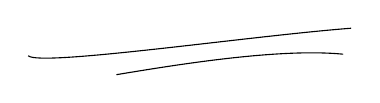
\begin{tikzpicture}[x=1cm,y=1cm]
\draw (0,0.06) .. controls (0.15,-0.08) and (2.8,0.31) .. (4.1,0.41);
\draw (1.12,-0.18) .. controls (1.9,-0.05) and (3.2,0.16) .. (4.0,0.08);
\end{tikzpicture}}
\scanpage{60}\mspage{59}
J'en viens à \unsure{des|du} \uline{\unsure{axiomes|axiome} de disjonction}
(At 8 était l' ``axiome des lieux'').

Notons d'abord

\deleted{\uline{At} 9} \deleted{Soient $\unsure{X|F}$}

\uline{Proposition} Soit $\unsure{\mathcal F|F}$ un atelier
At 1 -- At 3 (on \unsure{ne|n'y} va pas utiliser $\ll$).
Soient $F$ et $G\in\mathcal F$, alors $\unsure{\overline{1}|T|\mathrm{I}}$
% slanted
\margin{\unsure{Remarquons|Remarquer} \unsure{tt de suite} que $X\parallel Y\Longrightarrow\operatorname{Omb}(X)\cap\operatorname{Omb}Y=\varnothing$ a fortiori $\operatorname{omb}(X)\cap\operatorname{omb}(Y)=0$}
\[
F\parallel G\quad\Longleftrightarrow\quad\forall X\in\widetilde F,Y\in\widetilde G,\qquad X\parallel Y.
\]
Immédiat. \unsure{Egalmt|Egalement}, \deleted{\unsure{on trouve}} \inserted{on voudrait}

\begingroup\makeatletter\tagsleft@true\makeatother
\[
\begin{aligned}
&\text{\deleted{\uline{Proposition}} \deleted{\unsure{Corollaire}} Si }\ F\parallel G,\quad F'\ll F,\ G'\ll G,\\
&\text{alors }\ F'\parallel G'.
\end{aligned}
\tag*{(1.58)}
\]
\endgroup

En effet, \deleted{\unsure{il suffit|il soit}} on est ramené au cas où
$F'=X',\ G'=Y'$ \inserted{(\unsure{par prop})}, puis au cas
$F=X,\ G=Y$, en utilisant At 4.
% slanted
\margin{\uline{NB} Le seul pb, c'est de prouver que $F'\mathrel{\tikz[baseline=-.45ex,x=1em,y=1em]{\draw[line width=.055em] (.52,.27)--(.05,.055)--(.48,-.11); \draw[line width=.055em] (.14,.21)--(.46,.04)--(0,-.17);}}G'$ \deleted{\unsure{quand}} \deleted{\unsure{une fois cela vu}}, \inserted{\unsure{c'est ``oui''|c'est ``que''}}, $F'\overset{-\,\searrow}{\parallel}G'$. \deleted{\unsure{c'est ici|c'est lui}} Car sinon \unsure{car, un|car, le} $Z\in M$ \deleted{$Z$} avec $Z\leq F',\ Z\leq G'$ donne $Z\ll F,\ Z\ll G$ Or \deleted{dans} $\unsure{\widetilde{F\vee G}|\widehat{F\vee G}}$ les \unsure{4|2} relations $\ll$ et $\leq$ \unsure{coïncident}, de $\parallel$ \unsure{c.a.d.} le $\operatorname{Inf}$ pour $\leq$ $\unsure{\nexists|\neq}$, et pour $\ll$ on trouve absurdité\ldots}

Même, dans le cas ensembliste à figures de t.f.
(et $=$ finies) cela ne semble pas résulter
des autres axiomes -- cf page 55,
\unsure{Atens tf|Atens t.f|Atensfig} 3 nous dit quelles conditions
mettre à la relation $\underset{M}{\mathrel{\tikz[baseline=-.45ex,x=1em,y=1em]{\draw[line width=.055em] (.52,.27)--(.05,.055)--(.48,-.11); \draw[line width=.055em] (.14,.21)--(.46,.04)--(0,-.17);}}}$ \deleted{\unsure{de pré}} : d'être
stable par passage aux sous-strates, et
d' \deleted{être} plus forte que la relation $\underset{\mathrm{ens}}{\mathrel{\tikz[baseline=-.45ex,x=1em,y=1em]{\draw[line width=.055em] (.52,.27)--(.05,.055)--(.48,-.11); \draw[line width=.055em] (.14,.21)--(.46,.04)--(0,-.17);}}}$.
\scanpage{61}\mspage{60}
Or ça n'a pas l'air d'impliquer la condition.
Car ça n'implique pas que \deleted{la disjonction}
la disjonction ensembliste implique la disjonction géométrique. Prenons p.ex.
$M$ réduit à \deleted{\unsure{trois}} \inserted{des} multistrates \deleted{\unsure{chacune}}
réduites à une seule \deleted{ensemble} \inserted{strate} (ce qui
rend vide la première condition \unsure{Atens tf|Atens t.f|Atensfig} 3)
par exemple définies par les \deleted{\unsure{d|t}}trois ensembles
$A,B$ et $\unsure{A'|A}$, $A'\subsetneq A,\ A\cap B=\varnothing$. \deleted{Prenons}
\deleted{\unsure{donc}} $X=\{A\},\quad Y=\{B\},\quad X'=\{A'\}$, et soit $Y'=Y$,
donc $X'\deleted{\unsure{<|\leq}}\ll X,\quad Y'=Y$ donc $Y'\ll Y$. \deleted{On définit} \inserted{La}
\deleted{$\underset{M}{\mathrel{\tikz[baseline=-.45ex,x=1em,y=1em]{\draw[line width=.055em] (.52,.27)--(.05,.055)--(.48,-.11); \draw[line width=.055em] (.14,.21)--(.46,.04)--(0,-.17);}}}$ \unsure{comme étant la|comme étant la co}} \inserted{compatibilité ensembliste} des trois
multistrates est déjà acquise. Donc on
peut prendre pour $\underset{M}{\mathrel{\tikz[baseline=-.45ex,x=1em,y=1em]{\draw[line width=.055em] (.52,.27)--(.05,.055)--(.48,-.11); \draw[line width=.055em] (.14,.21)--(.46,.04)--(0,-.17);}}}$ n'importe quelle
relation \unsure{sym. refl|sym. réfl|sym. rfl}, \deleted{\unsure{donc}} \inserted{correspondant à} n'importe quelle
partie \deleted{\unsure{à deux éléments}} \deleted{\unsure{des}}\unsure{de} l'ens des
trois paires de \deleted{strates} multistrates $X,Y,X'$
on choisira $X\underset{M}{\mathrel{\tikz[baseline=-.45ex,x=1em,y=1em]{\draw[line width=.055em] (.52,.27)--(.05,.055)--(.48,-.11); \draw[line width=.055em] (.14,.21)--(.46,.04)--(0,-.17);}}}Y$, et $X'\underset{M}{\overline{\mathrel{\tikz[baseline=-.45ex,x=1em,y=1em]{\draw[line width=.055em] (.52,.27)--(.05,.055)--(.48,-.11); \draw[line width=.055em] (.14,.21)--(.46,.04)--(0,-.17);}}}}Y$ --
alors $X\underset{\unsure{\mathcal F|F}}{\parallel}Y$, mais $X'\underset{\mathcal F}{\overline{\parallel}}Y$, ok.

On posera donc
\begingroup\makeatletter\tagsleft@true\makeatother
\[
\begin{aligned}
&\text{\deleted{\uline{At} \uline{9}} Si }\ X,Y\ \deleted{\unsure{\in M}}\,,\ X',Y'\in M,\\
&\text{avec }\ X'\ll X,\quad Y'\ll Y,\quad \text{et si }X\parallel Y,\\
&\text{alors }\ X'\parallel Y'\quad(\text{il suffit de poser }X \mathrel{\tikz[baseline=-.45ex,x=1em,y=1em]{\draw[line width=.055em] (.52,.27)--(.05,.055)--(.48,-.11); \draw[line width=.055em] (.14,.21)--(.46,.04)--(0,-.17);}} Y)
\end{aligned}
\tag*{($*$)}
\]
\endgroup
\scanpage{62}\mspage{61}
mais je ne veux pas l'expliciter en
axiome à part ici, car je le vois comme
cas particulier d'un \uline{axiome de recollement \unsure{des|de} raffinements}, beaucoup
plus général, dont il sera question
plus bas. C'est un axiome qui s'énonce
sans référence particulière aux lieux.
Mais j'ai envie de \unsure{hasarder} deux
axiomes, impliquant encore les lieux.

% slanted
\margin{\unsure{Critère|Critére} de disjonction par les lieux.}
\uline{At} 9 Soient $X$ et $Y\in M$, telles que
$\forall x\in\operatorname{\underline{o}mb}(X),\ y\in\operatorname{\unsure{Omb|omb}}(Y)$, $x$ et $y$ soient
disjoints : \deleted{\unsure{i.e.} $x \mathrel{\tikz[baseline=-.45ex,x=1em,y=1em]{\draw[line width=.055em] (.52,.27)--(.05,.055)--(.48,-.11); \draw[line width=.055em] (.14,.21)--(.46,.04)--(0,-.17);}} y$.} $x\parallel y$. Alors \inserted{et alors \unsure{seult|seulement}} $X$ et $Y$
le sont $\quad X\parallel Y$.

D'autre part, pour un atelier ensembliste,
(et pas seulement \unsure{quasiensembliste|quasi ensembliste}!) on pose

\[
\text{\uline{Atens 2}\quad Si }\ x,y\in L,\ x\ne y,\quad \text{alors }\ x\underset{M}{\mathrel{\tikz[baseline=-.45ex,x=1em,y=1em]{\draw[line width=.055em] (.52,.27)--(.05,.055)--(.48,-.11); \draw[line width=.055em] (.14,.21)--(.46,.04)--(0,-.17);}}}y
\]
qui se traduit en termes de \deleted{$\unsure{M|L}, \mathrel{\tikz[baseline=-.45ex,x=1em,y=1em]{\draw[line width=.055em] (.52,.27)--(.05,.055)--(.48,-.11); \draw[line width=.055em] (.14,.21)--(.46,.04)--(0,-.17);}}$}
$\unsure{.|-}\,M\subset\operatorname{Figel}(\deleted{\unsure{L|l}}L)$, et $\underset{M}{\mathrel{\tikz[baseline=-.45ex,x=1em,y=1em]{\draw[line width=.055em] (.52,.27)--(.05,.055)--(.48,-.11); \draw[line width=.055em] (.14,.21)--(.46,.04)--(0,-.17);}}}$, par
\[
\text{\uline{Atens\deleted{\unsure{é|*}}\,\deleted{\unsure{g|s}}\unsure{tf|t.f|fig} 4}}\qquad
\forall\,x\deleted{\unsure{\in|\,\in L}},y\in L,\ x\ne y,\quad \text{on a }\{\{x\}\}\underset{M}{\mathrel{\tikz[baseline=-.45ex,x=1em,y=1em]{\draw[line width=.055em] (.52,.27)--(.05,.055)--(.48,-.11); \draw[line width=.055em] (.14,.21)--(.46,.04)--(0,-.17);}}}\{\{y\}\}.
\]
\scanpage{63}\mspage{62}
Donc

\uline{Corollaire} Pour un atelier ensembliste

\noindent\begin{tabular}{@{}|p{.92\linewidth}@{}}
(satisfaisant \deleted{\unsure{At 8|At}} aussi At 9 et Atens 2)
Si $F,G$ sont deux figures, pour que
$F\parallel G$, il \unsure{f|f.} et S que $\forall x\in\operatorname{omb}X,y\in\operatorname{omb}Y$,
on ait $x\parallel y$. \deleted{\unsure{ou encore}}
\end{tabular}

Dans le cas des ateliers \unsure{quelconque|quelconques}, on
trouve d'autre part.

\noindent\begin{tabular}{@{}|p{.92\linewidth}@{}}
\uline{Corollaire} Validité de $(1.58)$, si $\unsure{\mathcal F|F}$
satisfait At 9
\end{tabular}

D'autre part, je voudrais en présenter
un axiome facultatif

% slanted
\margin{\uline{NB} dans $\mathcal F$, le $\operatorname{Inf}$ \deleted{\unsure{de non|d'non}} vide existe tjrs, \unsure{$=$} \deleted{\unsure{pour}} $F\cap G$ sur $F,G$ \unsure{compatibles|compatible}, il correspond à l'intersection des parties \deleted{de $M$ de} fermées de $M$ de la forme $\widetilde F$. L'énoncé ci-contre s'étend \unsure{automatiquement} au cas de deux figures quelconques\ldots}
\uline{At \deleted{\unsure{ens fig|ensfiltr}}} \unsure{9$'$|91} Soient $X,Y\in M$, \deleted{$\unsure{F|E}$} et
soit \deleted{\unsure{au sens|on aura}} $F=X\cap Y$ \inserted{(donc $\widetilde F$ est} l'ens des strates communes).
\deleted{\unsure{qui est une partie fermée de} $M$,}
\inserted{Supposons que pour tout}
$x\in\operatorname{omb}(X)\unsure{\setminus|-}\operatorname{omb}(F)$ et tout $y\in\operatorname{omb}(Y)-\operatorname{omb}(F)$
on ait $x\unsure{\mathrel{\tikz[baseline=-.46ex,x=.68em,y=.68em]{\draw[line width=.075em] (.16,.64)--(.18,-.23) (.36,.67)--(.39,-.24) (.15,.23)--(.55,.22);}}|\parallel|\nparallel}y$ (donc $x\ne y$) $[$ce \unsure{que|qui}
\unsure{explique|implique} encore que \deleted{\unsure{on ait}}
\[
\operatorname{omb}(X)\cap\operatorname{omb}(Y)=\operatorname{omb}(F)\ \bigr]
\]
\diagram{\begin{tikzcd}[ampersand replacement=\&,column sep=small,row sep=small]
\operatorname{om}(X)\arrow[dr] \& \& \operatorname{omb}(Y)\arrow[dl,bend right=10]\\
\& \operatorname{omb}(F) \&
\end{tikzcd}}
Alors $X \mathrel{\tikz[baseline=-.45ex,x=1em,y=1em]{\draw[line width=.055em] (.52,.27)--(.05,.055)--(.48,-.11); \draw[line width=.055em] (.14,.21)--(.46,.04)--(0,-.17);}} Y$
\margin{\tikz[baseline=(note.base)]{\node[inner sep=2pt,outer sep=0pt,text width=\dimexpr\marginparwidth-4pt\relax,align=left] (note) {\uline{NB} la réciproque \deleted{\unsure{sera|être}}\unsure{reste|sera} vraie aussi, par axiome de disjonction plus bas p.72}; \draw[rounded corners=4pt] (note.north west)--(note.south west)--(note.south east);}}

Cet axiome est \unsure{``|''}\deleted{\unsure{in}}\unsure{intéressant}, en ce
qu'il exprime \deleted{\unsure{les|la}} compatibilité \inserted{$\mathrel{\tikz[baseline=-.45ex,x=1em,y=1em]{\draw[line width=.055em] (.52,.27)--(.05,.055)--(.48,-.11); \draw[line width=.055em] (.14,.21)--(.46,.04)--(0,-.17);}}$} des multistrates
génér\unsure{ales|iques} (qui \inserted{\unsure{pratiquement}} est un des \deleted{\unsure{grands points d'interrogation}}
\scanpage{64}\mspage{63}
ingrédients principaux pour décrire l'atelier, via $(M,\leq,\ll,\mathrel{\tikz[baseline=-.45ex,x=1em,y=1em]{\draw[line width=.055em] (.52,.27)--(.05,.055)--(.48,-.11); \draw[line width=.055em] (.14,.21)--(.46,.04)--(0,-.17);}})$) en termes
ensemblistes, au moyen de la seule
relation $\mathrel{\tikz[baseline=-.45ex,x=1em,y=1em]{\draw[line width=.055em] (.52,.27)--(.05,.055)--(.48,-.11); \draw[line width=.055em] (.14,.21)--(.46,.04)--(0,-.17);}}$ dans $L$ (puisque
\deleted{\unsure{si|il}} il est clair que pour deux \uline{lieux},
\begingroup\makeatletter\tagsleft@true\makeatother
\[
x\parallel y\quad\Longleftrightarrow\quad x \mathrel{\tikz[baseline=-.45ex,x=1em,y=1em]{\draw[line width=.055em] (.52,.27)--(.05,.055)--(.48,-.11); \draw[line width=.055em] (.14,.21)--(.46,.04)--(0,-.17);}} y\quad\text{et}\quad x\ne y
\tag*{(1.59)}
\]
\endgroup

\deleted{Le seul}
Cela mettrait donc un poids particulier
sur cette relation de $\underset{\unsure{L|\alpha}}{\mathrel{\tikz[baseline=-.45ex,x=1em,y=1em]{\draw[line width=.055em] (.52,.27)--(.05,.055)--(.48,-.11); \draw[line width=.055em] (.14,.21)--(.46,.04)--(0,-.17);}}}$ (ou ce qui
revient au $=\quad\underset{L}{\parallel}$) \uline{\deleted{\unsure{de|dans}}\unsure{dans}} $L$. Cet
\unsure{axiome} est bien raisonnable, y
compris dans des cas non ``ensembliste'',
mais le seul hic, c'est que il n'est
\uline{pas} satisfait dans les cas simpliciaux
les plus importants, cf exemples page \ldots.
Mais dans ce cas, on peut se rabattre sur
une \deleted{\unsure{propriét|propriété}} propriété qui fera le $=$
usage

% slanted
\margin{Variante ``simpliciale'' de \uline{At} 9$'$}
\uline{At \deleted{\unsure{fac|fer}}} \uline{9}$''$ Soient $X,Y\in M$ et $F$ comme
dans \unsure{Atfer|Atfac} 1. Alors
\[
X \mathrel{\tikz[baseline=-.45ex,x=1em,y=1em]{\draw[line width=.055em] (.52,.27)--(.05,.055)--(.48,-.11); \draw[line width=.055em] (.14,.21)--(.46,.04)--(0,-.17);}} Y\ \Longleftrightarrow\
\left\{\begin{aligned}
&\forall x\in\operatorname{omb}X\setminus\operatorname{omb}F\quad\text{et}\quad y\in\operatorname{om}Y\setminus\operatorname{omb}F,\\
&\hspace{9em}\text{on a }\ x\parallel y\\
&F\ \text{est \inserted{vide ou est} ``élémentaire'' (i.e. }F\in M\\
&\qquad\text{\unsure{(i.e.|i.e.} c'est une multistrate commune).}
\end{aligned}\right.
\]
\margin{\tikz[baseline=(note.base)]{\node[inner sep=2pt,outer sep=0pt,text width=\dimexpr\marginparwidth-4pt\relax,align=left] (note) {\uline{NB} On peut donner \unsure{variantes|variante} avec toute autre condition, sur l'ens ordonné $\widetilde F$.}; \draw[rounded corners=4pt] (note.north west)--(note.north east)--(note.south east);}}
\scanpage{65}\mspage{64}

Notons que \uline{At} 9 est impliqué par chacun des deux \deleted{\unsure{A|a}}axiomes At 9$'$, At 9$''$. \deleted{Et il le \unsure{sera|serait} aussi \unsure{par} l'axiome de recollement plus bas, \unsure{donc il} n'est pas tellement crucial en lui-même.}
% slanted
\margin{\textcircled{$*$} \unsure{Intervertir|Intervention} At 9, At 10, pour \unsure{bloquer} les \unsure{ens} At 8, At 10 (qui sont \unsure{les|des} \unsure{2|7} axiomes \deleted{d'existence} portant sur les strates ouvertes : l'existence des lieux et des \unsure{0-sphères|o-sphères} \unsure{reliées|reliés} aux \unsure{strates} \unsure{ouvertes|issues de}\unsure{.|)}}
% slanted
\margin{\unsure{Donner|Donnons} ici deuxième Axiome de \unsure{disjonction} \uline{At 10} Soient $\deleted{\unsure{x|X}}X,\deleted{\unsure{y|Y}}Y\in M$ \inserted{$X \mathrel{\tikz[baseline=-.45ex,x=1em,y=1em]{\draw[line width=.055em] (.52,.27)--(.05,.055)--(.48,-.11); \draw[line width=.055em] (.14,.21)--(.46,.04)--(0,-.17);}} Y$} \deleted{une figure, $\unsure{x,y}\in\operatorname{omb}(F)$} $X\ne Y$, \inserted{alors} \deleted{\unsure{appartenant à|appart. à|portent} des \uline{strates} \uline{ouvertes} \uline{disjointes}} tout $x\in\operatorname{omb}(X)^{\unsure{\circ|0}}$ \deleted{\unsure{i.e.} $\unsure{\exists x_i|X_i}$} est \uline{disjoint} de tout $y\in\operatorname{omb}(Y)^{\circ}$.}
% slanted
\margin{\uline{NB} Le cas où \deleted{$Y\unsure{\leq|\nleq}X$ ou $X\leq Y$ est} $X\wedge Y\ne X,Y$ résulterait aussi de l'axiome de recollement At 11 plus bas -- donc le cas crucial est celui où $Y\subset X$.}
% slanted
\margin{Les axiomes At 8, At 9, At 10 s'appelleront ``axiomes des lieux''.}
% slanted
\margin{\uline{At 10} $X,Y\in M$, $X\ne Y$ \inserted{$x,y\in\unsure{L|\mathcal L|\alpha}$} $x\overset{\circ}{\ll}X,\ y\overset{\circ}{\ll}Y\ \Longrightarrow\ x\parallel y$ (ou encore $x \mathrel{\tikz[baseline=-.45ex,x=1em,y=1em]{\draw[line width=.055em] (.52,.27)--(.05,.055)--(.48,-.11); \draw[line width=.055em] (.14,.21)--(.46,.04)--(0,-.17);}} y$, cela revient au $=$) Voir (\unsure{ci corr.|ci-contre}) p 72 \textcircled{$*$}}

\uline{21. juin}

\uline{Proposition} Soient $\unsure{\mathcal F|F}$ un atelier At 1 -- \deleted{\unsure{At 8|At 9}} At 7 $F\in\mathcal F$, $F'\ll F$, $G\leq F$. Alors
\[
G'=\operatorname{Inf}^{\ll}(F',G)
\]
existe, et $G'$ est une sous-figure de $F'$ : \deleted{On}
% slanted
\margin{Peut remonter avant les histoires de lieux}
\diagram{\begin{tikzcd}[ampersand replacement=\&,row sep=2.25em,column sep=2.2em]
F' \arrow[r,phantom,"\ll" description] \arrow[d,phantom,"{\rotatebox{90}{$\leq$}}" description] \& F \arrow[d,phantom,"{\rotatebox{90}{$\leq$}}" description]\\
G' \arrow[r,phantom,"\ll" description] \& G.
\end{tikzcd}}

On a
\begingroup\makeatletter\tagsleft@true\makeatother
\[
\widetilde G'=\{X\in\widetilde F'\mid X\ll G\}\ \deleted{\unsure{=\operatorname{Inf}^{\leq}|=\operatorname{Inf}^{\ll}|\ll\operatorname{Inf}^{\leq}}}.\tag*{(1.60)}
\]
\endgroup
% slanted
\margin{Terminologie : \uline{Sous figure induite} $G'$ de $G$ par la sous-figure $F'$ de $F$. \uline{Raffinement} $G'$ de $G$, \uline{induit} sur la sous-figure $G$ de $F$ par le \unsure{raffinem.|raffinement} $F'$ de $F$, ou $F'/G$ \unsure{--|.}}

\uline{Démonstration} La formule (1.60) \deleted{résulte} \inserted{est} tautologique par la définition des $\operatorname{Inf}^{\ll}$ et du fait que $\leq$ implique $\ll$. Mais sans admettre l'existence du $\operatorname{Inf}$, la formule (1.60) définit une partie fermée de $\widetilde F'$, donc une sous-figure $G'$ de $F'$, et on a évidemment $G\ll F$ par
